\documentclass{jfm}
\usepackage{graphicx}
\usepackage{epstopdf, epsfig}
\usepackage[caption=false]{subfig}

\newtheorem{lemma}{Lemma}
\newtheorem{corollary}{Corollary}

\shorttitle{}
\shortauthor{}

\title{Validation of actuator line algorithm through simulation of
  flow past an elliptic wing}

\author{Ganesh Vijayakumar}

\begin{document}

\maketitle

\begin{abstract}
The objective of this work is to document the validation of the
actuator line algorithm in Nalu through simulation of the flow past an
elliptic wing. 
\end{abstract}

\section{Introduction}
\label{sec:intro}
We plan to validate the implementation of the actuator line algorithm in Nalu
\citep{naluDoc} against the solution using lifting line theory. The
elliptic wing is modeled using OpenFAST \citep{OpenFAST:2017}, a
aero-hydro-servo-elastic tool to model wind turbines developed by the
National Renewable Energy Laboratory (NREL). A static wind turbine
model was created in OpenFAST with just one elliptic wing and all
other systems including structural deformation, controls, etc. are turned off.

\section{Lifting line theory}
\label{sec:ll_soln}

The elliptic wing simulated in this work is an infinitesimally thin wing
with a maximum chord ($c_0$) of $1m$ and an aspect ratio
($b/c_0$) of 10.0. The lift-curve slope ($d C_l/d \alpha$) of all airfoil sections on
the wing is assumed to be $2 \pi$ with no pressure or viscous drag. Using lifting line theory \citep{KatzPlotkin:2002}, the loads on the elliptic wing are

\begin{eqnarray}
\textrm{Area } S &=& \pi \frac{c_0}{2} \frac{b}{2},\\
\textrm{Maximum circulation } \Gamma_{\mathrm{max}} &=& \frac{2 b
                                                     U_{\infty}
                                                     (\alpha -
                                                     \alpha_{L0})}{1 +
                                                     4b/2\pi
                                                     c_0},\\
\textrm{Lift coefficient } C_L & \equiv & \frac{L}{0.5 \rho U_{\infty}^2
                                 S} = \frac{\pi}{2} \frac{b}{S}
                                 \frac{\Gamma_{\mathrm{max}}}{U_{\infty}},\\
\textrm{Lift coefficient } C_D & \equiv & \frac{D}{0.5 \rho U_{\infty}^2
                                 S} = \frac{\pi}{4S} \frac{\Gamma_{\mathrm{max}}^2}{U_{\infty}^2},\\
\textrm{Constant induced downwash } w_i &=&
                                          \frac{\Gamma_{\mathrm{max}}}{2b}.
\end{eqnarray}

\section{Details of numerical simulations}


\begin{figure}
  \centerline{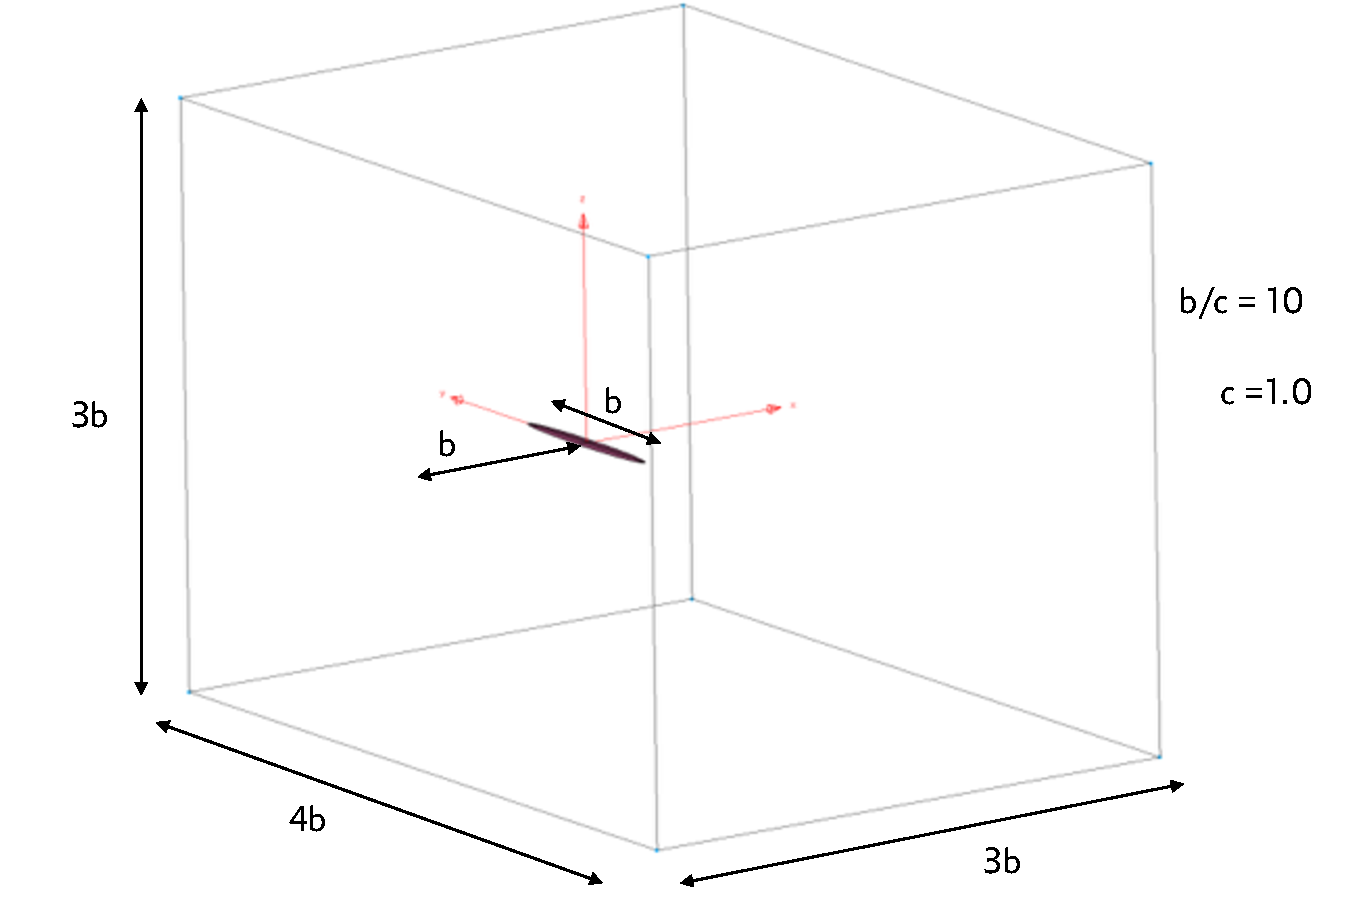
\includegraphics[width=\textwidth]{images/domain_illustration}}% Images in 100% size
  \caption{Illustration of the domain used to simulate the flow past
    an elliptic wing at a constant angle of attack. The wing is shown
    only for purposes of illustration and is modeled in the code using
  the method of actuator lines.}
\label{fig:domain_illustration}
\end{figure}

\begin{eqnarray}  
  \textrm{Span: } & 10m \nonumber \\
  \textrm{Max chord: } & 1.0m \nonumber \\
  \textrm{Angle of attack: } & 7^{\circ} \nonumber \\
  U_{\infty} \textrm{: } & 10.0m/s \label{eqn:sim_parameters} \\
  \Rey \textrm{ based on chord: } & 0.66M \nonumber \\
  \textrm{Number of actuator points across span: } & 50 \nonumber
\end{eqnarray}


The flow past the elliptic wing is simulated in a domain shown in
figure \ref{fig:domain_illustration}. The choice of domain size is based on
the recommendation by Tony Martinez. Some parameters of the simulation
are described in equation \ref{eqn:sim_parameters}. As described in the
Nalu theory manual \citep{naluDoc}, the actuator line algorithm solves
equation \ref{eqn:mom-ns-bodyforce}, where $\epsilon$ is the spreading
width. It is necessary to maintain a constant $\epsilon$ to observe
convergence of the solution with grid refinement. However, we do
expect the solution from the actuator line algorithm to be closer to
that from lifting line theory with reducing $\epsilon$. Hence,
we perform five numerical simulations with grid resolutions as shown
in table \ref{tab:gr}. Simulations \textit{a,b,c} use $\epsilon=1m$ and
\textit{d,e} use $\epsilon=0.5m$. We expect to see grid convergence
with simulations \textit{a,b,c} while we expect simulations
\textit{d,e} to predict a solution closer to the lifting line solution
compared to simulations \textit{a,b,c}.


\begin{eqnarray}
 \int \frac{\partial \bar{\rho} \tilde{u}_i} {\partial t} {\rm d}V
 + \int \bar{\rho} \tilde{u}_i \tilde{u}_j n_j {\rm d}S 
 + \int \bar{P} n_i {\rm d}S &=& \int \bar{\tau}_{ij} n_j {\rm d}S 
 + \int \tau_{u_i u_j} n_j {\rm d}S  
 + \int \left(\bar{\rho} - \rho_{\circ} \right) g_i {\rm d}V \nonumber \\
 & & \qquad \qquad + \int \left ( \sum_{k=0}^N g(\vec{r}^k) F_i^k  \right ) {\rm d}V,  \label{eqn:mom-ns-bodyforce} \\
\textrm{where } g(\vec{r}) &=& \frac{1}{\pi^{3/2} \epsilon^3} e^{-\left( \left| \vec{r}
  \right|/\epsilon \right)^2}.
\end{eqnarray}


\begin{table}
  \begin{center}
\def~{\hphantom{0}}
  \begin{tabular}{lccc}
      Case & $\Delta x/c_0$  & $\Delta t$ & $\epsilon/\Delta$ \\[3pt]
      \textit{a} &  0.125 & 0.00125 & 8.0 \\
      \textit{b} &  0.25  & 0.0025  & 4.0 \\
      \textit{c} &  0.5   & 0.005   & 2.0 \\
      \textit{d} &  0.125 & 0.00125 & 4.0 \\
      \textit{e} &  0.25 & 0.0025   & 2.0 \\
  \end{tabular}
  \caption{Grid resolution and actuator force spreading width
    $\epsilon$ for different numerical simulations.}
  \label{tab:gr}
  \end{center}
\end{table}


\section{Results}


The data shown in figures \ref{fig:CL_CD}-\ref{fig:aoa} are computed
purely using output from OpenFAST. Unfortunately OpenFAST can only
output data at a maximum of 9 stations along the blade. For this specific work, I
had designed the aerodynamics module (AeroDyn) inside OpenFAST to use
18 stations to compute the forces along the blade. However, the mesh
mapping algorithm in OpenFAST is used to interpolate the forces per
unit length along the blade into discrete point forces at 50 actuator
points along the blade as described in equation \ref{eqn:sim_parameters}.

Figure \ref{fig:CL_CD} shows the comparsion of lift and drag
coefficient predicted by the actuator line simulations to the solution
from lifting line theory. Simulations \textit{d} and \textit{e} are closer to the
lifting line solution compared to \textit{a,b,c} because of the
smaller $\epsilon$. Simulations \textit{a,b,c} show grid convergence
since they use the same $\epsilon$. Figure \ref{fig:lpul_dpul} show
similar results through the span wise distribution of the lift and
drag per unit length along the blade. Figure \ref{fig:aoa} shows the
comparison of the predicted angle of attack on the blade to the
constant angle attack predicted by the lifting line theory. As
expected, the agreement with the lifting line theory is much better near the
mid-span region compared to the wing tips. Figure \ref{fig:act_l_act_d}
shows the discrete point forces at the actuator points on the blade.

\begin{figure}
  \subfloat[\label{subfig:CL}]{%
    \includegraphics[width=0.45\textwidth]{../analysis/LiftCoeff.pdf}
  }
  \hfill
  \subfloat[\label{subfig:CD}]{%
    \includegraphics[width=0.45\textwidth]{../analysis/DragCoeff.pdf}
  }
  \caption{Comparison of (a) lift coefficient $C_L$ and (b) drag
    coeffficient $C_D$ for an elliptic wing simulated using actuator
    line algorithm to solution using lifting line theory.}
\label{fig:CL_CD}
\end{figure}


\begin{figure}
  \subfloat[\label{subfig:lpul}]{%
    \includegraphics[width=0.45\textwidth]{../analysis/LiftForcePerUnitLength.pdf}
  }
  \hfill
  \subfloat[\label{subfig:dpul}]{%
    \includegraphics[width=0.45\textwidth]{../analysis/DragForcePerUnitLength.pdf}
  }
  \caption{Comparison of (a) Lift force per unit length and (b) Drag force per unit
    length on an elliptic wing simulated using actuator line algorithm
  to solution using lifting line theory. Results are only shown at 9
  different stations along the blade that are output from OpenFAST.}
\label{fig:lpul_dpul}
\end{figure}

\begin{figure}
  \centerline{\includegraphics[width=\textwidth]{../analysis/AoA.pdf}}% Images in 100% size
  \caption{Comparison of angle of attack distribution on an elliptic
    wing simulated using actuator line algorithm to solution using
    lifting line theory. Results are only shown at 9
  different stations along the blade that are output from OpenFAST.}
\label{fig:aoa}
\end{figure}

\begin{figure}
  \subfloat[\label{subfig:act_l}]{%
    \includegraphics[width=0.45\textwidth]{../analysis/actuator_lift_force.pdf}
  }
  \hfill
  \subfloat[\label{subfig:act_d}]{%
    \includegraphics[width=0.45\textwidth]{../analysis/actuator_drag_force.pdf}
  }
  \caption{(a) Actuator lift force and (b) actuator drag force on an elliptic wing simulated using actuator line algorithm.}
\label{fig:act_l_act_d}
\end{figure}

\section{Conclusions}

The simulation of the flow past an elliptic wing at a constant angle
of attack using the actuator line algorithm boosts our confidence in
the implementation of the algorithm and the coupling to OpenFAST in
Nalu. The results from the numerical simulations show good agreement
with the solution from lifting line theory and convergence with mesh
refinement. As expected, the solution from the numerical simulations
also converges towards the lifting line solution as the spreading
width $\epsilon$ is reduced. Future work on implementing advanced
actuator line methods where the spreading function is not isotropic
and/or the spreading width $\epsilon$ is a function of the local chord
could help bring the solution closer to that from lifting line theory.

\bibliographystyle{jfm}
% Note the spaces between the initials
\bibliography{references}

\end{document}
